% Options for packages loaded elsewhere
\PassOptionsToPackage{unicode}{hyperref}
\PassOptionsToPackage{hyphens}{url}
\PassOptionsToPackage{dvipsnames,svgnames,x11names}{xcolor}
%
\documentclass[
]{article}
\usepackage{amsmath,amssymb}
\usepackage{iftex}
\ifPDFTeX
  \usepackage[T1]{fontenc}
  \usepackage[utf8]{inputenc}
  \usepackage{textcomp} % provide euro and other symbols
\else % if luatex or xetex
  \usepackage{unicode-math} % this also loads fontspec
  \defaultfontfeatures{Scale=MatchLowercase}
  \defaultfontfeatures[\rmfamily]{Ligatures=TeX,Scale=1}
\fi
\usepackage{lmodern}
\ifPDFTeX\else
  % xetex/luatex font selection
\fi
% Use upquote if available, for straight quotes in verbatim environments
\IfFileExists{upquote.sty}{\usepackage{upquote}}{}
\IfFileExists{microtype.sty}{% use microtype if available
  \usepackage[]{microtype}
  \UseMicrotypeSet[protrusion]{basicmath} % disable protrusion for tt fonts
}{}
\makeatletter
\@ifundefined{KOMAClassName}{% if non-KOMA class
  \IfFileExists{parskip.sty}{%
    \usepackage{parskip}
  }{% else
    \setlength{\parindent}{0pt}
    \setlength{\parskip}{6pt plus 2pt minus 1pt}}
}{% if KOMA class
  \KOMAoptions{parskip=half}}
\makeatother
\usepackage{xcolor}
\usepackage[margin=1in]{geometry}
\usepackage{color}
\usepackage{fancyvrb}
\newcommand{\VerbBar}{|}
\newcommand{\VERB}{\Verb[commandchars=\\\{\}]}
\DefineVerbatimEnvironment{Highlighting}{Verbatim}{commandchars=\\\{\}}
% Add ',fontsize=\small' for more characters per line
\usepackage{framed}
\definecolor{shadecolor}{RGB}{35,38,41}
\newenvironment{Shaded}{\begin{snugshade}}{\end{snugshade}}
\newcommand{\AlertTok}[1]{\textcolor[rgb]{0.58,0.85,0.30}{\textbf{\colorbox[rgb]{0.30,0.12,0.14}{#1}}}}
\newcommand{\AnnotationTok}[1]{\textcolor[rgb]{0.25,0.50,0.35}{#1}}
\newcommand{\AttributeTok}[1]{\textcolor[rgb]{0.16,0.50,0.73}{#1}}
\newcommand{\BaseNTok}[1]{\textcolor[rgb]{0.96,0.45,0.00}{#1}}
\newcommand{\BuiltInTok}[1]{\textcolor[rgb]{0.50,0.55,0.55}{#1}}
\newcommand{\CharTok}[1]{\textcolor[rgb]{0.24,0.68,0.91}{#1}}
\newcommand{\CommentTok}[1]{\textcolor[rgb]{0.48,0.49,0.49}{#1}}
\newcommand{\CommentVarTok}[1]{\textcolor[rgb]{0.50,0.55,0.55}{#1}}
\newcommand{\ConstantTok}[1]{\textcolor[rgb]{0.15,0.68,0.68}{\textbf{#1}}}
\newcommand{\ControlFlowTok}[1]{\textcolor[rgb]{0.99,0.74,0.29}{\textbf{#1}}}
\newcommand{\DataTypeTok}[1]{\textcolor[rgb]{0.16,0.50,0.73}{#1}}
\newcommand{\DecValTok}[1]{\textcolor[rgb]{0.96,0.45,0.00}{#1}}
\newcommand{\DocumentationTok}[1]{\textcolor[rgb]{0.64,0.20,0.25}{#1}}
\newcommand{\ErrorTok}[1]{\textcolor[rgb]{0.85,0.27,0.33}{\underline{#1}}}
\newcommand{\ExtensionTok}[1]{\textcolor[rgb]{0.00,0.60,1.00}{\textbf{#1}}}
\newcommand{\FloatTok}[1]{\textcolor[rgb]{0.96,0.45,0.00}{#1}}
\newcommand{\FunctionTok}[1]{\textcolor[rgb]{0.56,0.27,0.68}{#1}}
\newcommand{\ImportTok}[1]{\textcolor[rgb]{0.15,0.68,0.38}{#1}}
\newcommand{\InformationTok}[1]{\textcolor[rgb]{0.77,0.36,0.00}{#1}}
\newcommand{\KeywordTok}[1]{\textcolor[rgb]{0.81,0.81,0.76}{\textbf{#1}}}
\newcommand{\NormalTok}[1]{\textcolor[rgb]{0.81,0.81,0.76}{#1}}
\newcommand{\OperatorTok}[1]{\textcolor[rgb]{0.81,0.81,0.76}{#1}}
\newcommand{\OtherTok}[1]{\textcolor[rgb]{0.15,0.68,0.38}{#1}}
\newcommand{\PreprocessorTok}[1]{\textcolor[rgb]{0.15,0.68,0.38}{#1}}
\newcommand{\RegionMarkerTok}[1]{\textcolor[rgb]{0.16,0.50,0.73}{\colorbox[rgb]{0.08,0.19,0.26}{#1}}}
\newcommand{\SpecialCharTok}[1]{\textcolor[rgb]{0.24,0.68,0.91}{#1}}
\newcommand{\SpecialStringTok}[1]{\textcolor[rgb]{0.85,0.27,0.33}{#1}}
\newcommand{\StringTok}[1]{\textcolor[rgb]{0.96,0.31,0.31}{#1}}
\newcommand{\VariableTok}[1]{\textcolor[rgb]{0.15,0.68,0.68}{#1}}
\newcommand{\VerbatimStringTok}[1]{\textcolor[rgb]{0.85,0.27,0.33}{#1}}
\newcommand{\WarningTok}[1]{\textcolor[rgb]{0.85,0.27,0.33}{#1}}
\usepackage{longtable,booktabs,array}
\usepackage{calc} % for calculating minipage widths
% Correct order of tables after \paragraph or \subparagraph
\usepackage{etoolbox}
\makeatletter
\patchcmd\longtable{\par}{\if@noskipsec\mbox{}\fi\par}{}{}
\makeatother
% Allow footnotes in longtable head/foot
\IfFileExists{footnotehyper.sty}{\usepackage{footnotehyper}}{\usepackage{footnote}}
\makesavenoteenv{longtable}
\usepackage{graphicx}
\makeatletter
\def\maxwidth{\ifdim\Gin@nat@width>\linewidth\linewidth\else\Gin@nat@width\fi}
\def\maxheight{\ifdim\Gin@nat@height>\textheight\textheight\else\Gin@nat@height\fi}
\makeatother
% Scale images if necessary, so that they will not overflow the page
% margins by default, and it is still possible to overwrite the defaults
% using explicit options in \includegraphics[width, height, ...]{}
\setkeys{Gin}{width=\maxwidth,height=\maxheight,keepaspectratio}
% Set default figure placement to htbp
\makeatletter
\def\fps@figure{htbp}
\makeatother
\setlength{\emergencystretch}{3em} % prevent overfull lines
\providecommand{\tightlist}{%
  \setlength{\itemsep}{0pt}\setlength{\parskip}{0pt}}
\setcounter{secnumdepth}{5}
\usepackage[english]{babel}
\usepackage{natbib}
\usepackage{url}
\usepackage{amsmath}
\usepackage{graphicx}
\usepackage{parskip}
\usepackage{fancyhdr}
\usepackage{vmargin}
\setmarginsrb{3 cm}{2.5 cm}{3 cm}{2.5 cm}{1 cm}{1.5 cm}{1 cm}{1.5 cm}
\usepackage{float}
\pagestyle{fancy}
\fancyhf{}
\rhead{FLXETH002 \& FRNBEN003}
\lhead{Analytics A2}
\cfoot{\thepage}
\ifLuaTeX
  \usepackage{selnolig}  % disable illegal ligatures
\fi
\IfFileExists{bookmark.sty}{\usepackage{bookmark}}{\usepackage{hyperref}}
\IfFileExists{xurl.sty}{\usepackage{xurl}}{} % add URL line breaks if available
\urlstyle{same}
\hypersetup{
  colorlinks=true,
  linkcolor={blue},
  filecolor={Maroon},
  citecolor={blue},
  urlcolor={blue},
  pdfcreator={LaTeX via pandoc}}

\author{}
\date{\vspace{-2.5em}}

\begin{document}

\begin{titlepage}
    \centering
    % Ensure uct-logo.png is in your working directory or provide the full path
    \includegraphics[width = 6cm]{uct-logo.png}\\[1.0 cm]
    \vspace*{0.5 cm}
    \textsc{\LARGE University of Cape Town}\\[2.0 cm]
    \textsc{\Large STA4010W}\\[0.5 cm]
    \textsc{\large Analytics}\\[0.5 cm]
    \rule{\linewidth}{0.2 mm} \\[0.4 cm]
    { \huge \bfseries Assessment 2: Neural Networks}\\
    \rule{\linewidth}{0.2 mm} \\[1.5 cm]
    
    \begin{minipage}{0.4\textwidth}
        \begin{flushleft} \large
            \emph{Author:}\\
            Ethon Felix \\
            Benjamin Franco
            \end{flushleft}
            \end{minipage}~
            \begin{minipage}{0.4\textwidth}
            \begin{flushright} \large
            \emph{Student Number:} \\
            FLXETH002 \\
            FRNBEN003
        \end{flushright}
    \end{minipage}\\[2 cm]
    
    {\large 20 April 2026}\\[2 cm]
    \vfill
\end{titlepage}

\newpage

\begin{enumerate}
\def\labelenumi{\alph{enumi}.}
\tightlist
\item
  Conduct an EDA by plotting input-response relationships and comment on
  whether a neural network is an appropriate model class.
\end{enumerate}

\vspace{0.2cm}

\begin{Shaded}
\begin{Highlighting}[]
\CommentTok{\# Read the data from the text file}
\NormalTok{data }\OtherTok{\textless{}{-}} \FunctionTok{read.table}\NormalTok{(}\StringTok{"HittingTheWall\_2026.txt"}\NormalTok{, }\AttributeTok{header =} \ConstantTok{TRUE}\NormalTok{)}


\CommentTok{\# Set up a 2 x 2 plotting grid}

\FunctionTok{par}\NormalTok{(}
  \AttributeTok{mfrow =} \FunctionTok{c}\NormalTok{(}\DecValTok{2}\NormalTok{, }\DecValTok{2}\NormalTok{),          }\CommentTok{\# 2x2 grid}
  \AttributeTok{mar   =} \FunctionTok{c}\NormalTok{(}\DecValTok{4}\NormalTok{, }\DecValTok{4}\NormalTok{, }\DecValTok{3}\NormalTok{, }\DecValTok{1}\NormalTok{),    }\CommentTok{\# bottom, left, top, right margins}
  \AttributeTok{oma   =} \FunctionTok{c}\NormalTok{(}\DecValTok{0}\NormalTok{, }\DecValTok{0}\NormalTok{, }\DecValTok{2}\NormalTok{, }\DecValTok{0}\NormalTok{),    }\CommentTok{\# outer margins for overall title}
  \AttributeTok{cex.main =} \FloatTok{0.8}\NormalTok{,          }\CommentTok{\# smaller plot titles}
  \AttributeTok{cex.lab  =} \FloatTok{0.8}\NormalTok{,          }\CommentTok{\# axis label size}
  \AttributeTok{cex.axis =} \FloatTok{0.9}            \CommentTok{\# axis tick label size}
\NormalTok{)}


\CommentTok{\# 1. Boxplot: Carbs vs Bombed}
\FunctionTok{boxplot}\NormalTok{(Carbs }\SpecialCharTok{\textasciitilde{}}\NormalTok{ Bombed,}
        \AttributeTok{data =}\NormalTok{ data,}
        \AttributeTok{col =} \FunctionTok{c}\NormalTok{(}\StringTok{"blue"}\NormalTok{, }\StringTok{"red"}\NormalTok{),}
        \AttributeTok{main =} \StringTok{"Carbohydrate Intake Vs. Bombed"}\NormalTok{,}
        \AttributeTok{xlab =} \StringTok{"Bombed"}\NormalTok{,}
        \AttributeTok{ylab =} \StringTok{"Carbintake (g/h)"}\NormalTok{,}
        \AttributeTok{border =} \StringTok{"black"}\NormalTok{)}

\CommentTok{\# 2. Boxplot: Fluid vs Bombed}
\FunctionTok{boxplot}\NormalTok{(Fluid }\SpecialCharTok{\textasciitilde{}}\NormalTok{ Bombed,}
        \AttributeTok{data =}\NormalTok{ data,}
        \AttributeTok{col =} \FunctionTok{c}\NormalTok{(}\StringTok{"blue"}\NormalTok{, }\StringTok{"red"}\NormalTok{),}
        \AttributeTok{main =} \StringTok{"Fluid Intake Vs. Bombed"}\NormalTok{,}
        \AttributeTok{xlab =} \StringTok{"Bombed"}\NormalTok{,}
        \AttributeTok{ylab =} \StringTok{"Fluid intake (L/h)"}\NormalTok{,}
        \AttributeTok{border =} \StringTok{"black"}\NormalTok{)}

\CommentTok{\# 3. Boxplot: AveSpeed vs Bombed}
\FunctionTok{boxplot}\NormalTok{(AveSpeed }\SpecialCharTok{\textasciitilde{}}\NormalTok{ Bombed,}
        \AttributeTok{data =}\NormalTok{ data,}
        \AttributeTok{col =} \FunctionTok{c}\NormalTok{(}\StringTok{"blue"}\NormalTok{, }\StringTok{"red"}\NormalTok{),}
        \AttributeTok{main =} \StringTok{"Average Speed by Bombing Status"}\NormalTok{,}
        \AttributeTok{xlab =} \StringTok{"Bombed"}\NormalTok{,}
        \AttributeTok{ylab =} \StringTok{"Average speed (km/h)"}\NormalTok{,}
        \AttributeTok{border =} \StringTok{"black"}\NormalTok{)}

\CommentTok{\# 4. Barplot: Proportion bombed by Sex}
\NormalTok{prop\_bombed }\OtherTok{\textless{}{-}} \FunctionTok{tapply}\NormalTok{(data}\SpecialCharTok{$}\NormalTok{Bombed }\SpecialCharTok{==} \StringTok{"TRUE"}\NormalTok{, data}\SpecialCharTok{$}\NormalTok{Sex, mean)}

\FunctionTok{barplot}\NormalTok{(prop\_bombed,}
        \AttributeTok{col =} \FunctionTok{c}\NormalTok{(}\StringTok{"blue"}\NormalTok{, }\StringTok{"red"}\NormalTok{),}
        \AttributeTok{ylim =} \FunctionTok{c}\NormalTok{(}\DecValTok{0}\NormalTok{, }\DecValTok{1}\NormalTok{),}
        \AttributeTok{main =} \StringTok{"Proportion Bombed by Sex"}\NormalTok{,}
        \AttributeTok{xlab =} \StringTok{"Sex"}\NormalTok{,}
        \AttributeTok{ylab =} \StringTok{"Proportion bombed"}\NormalTok{,}
        \AttributeTok{border =} \StringTok{"black"}\NormalTok{)}

\CommentTok{\# Add labels above bars}
\FunctionTok{text}\NormalTok{(}\AttributeTok{x =} \FunctionTok{c}\NormalTok{(}\FloatTok{0.7}\NormalTok{, }\FloatTok{1.9}\NormalTok{),}
     \AttributeTok{y =}\NormalTok{ prop\_bombed,}
     \AttributeTok{labels =} \FunctionTok{round}\NormalTok{(prop\_bombed, }\DecValTok{2}\NormalTok{),}
     \AttributeTok{pos =} \DecValTok{3}\NormalTok{)}

\CommentTok{\# Optional overall title}
\FunctionTok{mtext}\NormalTok{(}\StringTok{"Exploratory Data Analysis of Bombing Risk"}\NormalTok{, }\AttributeTok{outer =} \ConstantTok{TRUE}\NormalTok{, }\AttributeTok{cex =} \DecValTok{1}\NormalTok{, }\AttributeTok{font =} \DecValTok{2}\NormalTok{)}
\end{Highlighting}
\end{Shaded}

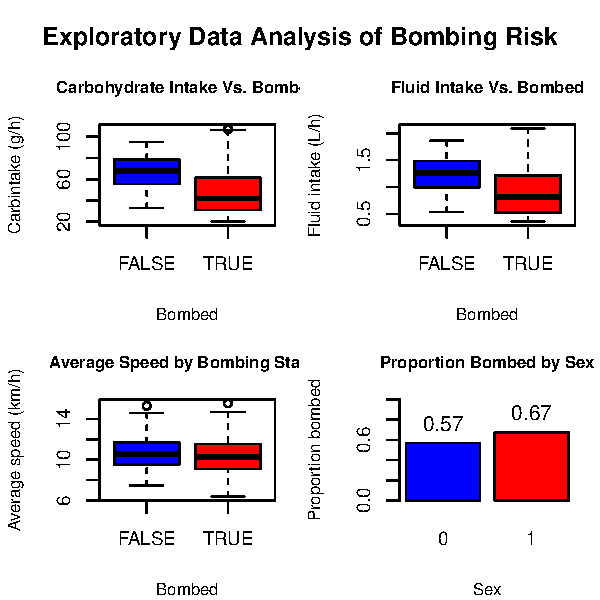
\includegraphics[width=0.8\linewidth]{Analytics-A2_files/figure-latex/unnamed-chunk-1-1}

Exploratory data analysis reveals several important patterns in the
dataset:

Carbohydrate Intake: The boxplot of Carbs intake versus Bombed status
shows that runners who bombed out during the race tended to have lower
carbohydrate intake per hour. There appears to be a threshold effect,
where bombing is much more likely below a certain level of carb intake,
supporting the need for a nonlinear model.

Fluid Intake: Similarly, the boxplot for Fluid intake indicates that
bombing out is associated with lower fluid intake per hour. The
relationship is not strictly linear, as there is considerable overlap
and possible threshold effects.

Sex: The bar plot of Bombed proportion by Sex demonstrates that a higher
proportion of males (67\%) bombed compared to females (57\%). This
suggests that sex may play a role in the likelihood of bombing, and
potential interactions should be considered.

Average Speed: The boxplot for AveSpeed shows little difference between
bombed and non-bombed groups, indicating that average speed is not a
strong predictor of bombing out in this sample.

The relationships between nutrition variables and bombing are not
strictly linear, with overlapping distributions, threshold effects, and
potential interactions. These findings suggest that a nonlinear model,
such as a neural network, is appropriate for capturing the complexity of
the data and providing more accurate predictions. \newpage

\begin{enumerate}
\def\labelenumi{\alph{enumi}.}
\setcounter{enumi}{1}
\tightlist
\item
\end{enumerate}

To show that

\[
\sigma(z_j) = \underbrace{\frac{\exp(z_j)}{\sum_{i=1}^q \exp(z_i)}}_\textbf{Eq. 1} =\underbrace{\frac{\exp(z_j - z^*)}{\sum_{i=1}^q \exp(z_i - z^*)}}_{\textbf{Eq. 2}} \quad \text{where } z^* = \max \{z_1,z_2,\dots,z_q\}
\] \vspace{0.2cm}

we start by expanding Equation 2 as follows

\[
\begin{aligned}
\frac{\exp(z_j - z^*)}{\sum_{i=1}^q \exp(z_i - z^*)} = \frac{\exp(z_j)\exp(-z^*)}{\sum_{i=1}^q \exp(z_i) \exp(- z^*)} = \frac{\exp(z_j)}{\sum_{i=1}^q \exp(z_i)}
\end{aligned}
\]

\vspace{0.2cm}

which shows that equations 1 and 2 are mathematically equivalent.

\vspace{0.2cm}

Subtracting the maximum logit \((z^*)\) ensures that the largest
exponent is zero and all others are negative, preventing overflow in the
exponential calculation. This makes the softmax calculation robust and
reliable for all input values. This is especially important in neural
networks and deep learning, where logits can be very large or very
small.

\begin{enumerate}
\def\labelenumi{\alph{enumi}.}
\setcounter{enumi}{2}
\tightlist
\item
\end{enumerate}

\begin{Shaded}
\begin{Highlighting}[]
\NormalTok{softmax }\OtherTok{=} \ControlFlowTok{function}\NormalTok{(X)\{}
\NormalTok{ max }\OtherTok{=} \FunctionTok{apply}\NormalTok{(X, }\DecValTok{2}\NormalTok{, max)}
\NormalTok{ X\_centered }\OtherTok{=}\NormalTok{ X}
 \ControlFlowTok{for}\NormalTok{ (i }\ControlFlowTok{in} \DecValTok{1}\SpecialCharTok{:}\FunctionTok{ncol}\NormalTok{(X))\{}
\NormalTok{   X\_centered[,i] }\OtherTok{=}\NormalTok{ X[,i]}\SpecialCharTok{{-}}\NormalTok{max[i]}
\NormalTok{ \}}
 
\NormalTok{ exp\_X }\OtherTok{=} \FunctionTok{exp}\NormalTok{(X\_centered)}
 
\NormalTok{ probs }\OtherTok{=}\NormalTok{ exp\_X}
\NormalTok{ col\_sums }\OtherTok{=} \FunctionTok{colSums}\NormalTok{(exp\_X)}
 \ControlFlowTok{for}\NormalTok{ (i }\ControlFlowTok{in} \DecValTok{1}\SpecialCharTok{:}\FunctionTok{ncol}\NormalTok{(exp\_X))\{}
\NormalTok{   probs[,}\DecValTok{1}\NormalTok{] }\OtherTok{=}\NormalTok{ exp\_X[,i]}\SpecialCharTok{/}\NormalTok{col\_sums[i]}
\NormalTok{ \}}
 
 \FunctionTok{return}\NormalTok{(probs)}
\NormalTok{\}}
\end{Highlighting}
\end{Shaded}

\begin{enumerate}
\def\labelenumi{\alph{enumi}.}
\setcounter{enumi}{3}
\tightlist
\item
\end{enumerate}

\textbf{Inputs:} - \(X^u\): Demographic input matrix (\(p^u \times N\))
- \(X^v\): Nutrition input matrix (\(p^v \times N\))

\textbf{First Hidden Layer (Split):} - \(W^u_1\): Weights for
\(u\)-hemisphere (\(m \times p^u\)) - \(b^u_1\): Biases for
\(u\)-hemisphere (\(m \times 1\)) - \(W^v_1\): Weights for
\(v\)-hemisphere (\(m \times p^v\)) - \(b^v_1\): Biases for
\(v\)-hemisphere (\(m \times 1\))

\textbf{Activations:} \[
A^u_1 = \tanh(W^u_1 X^u + b^u_1)
\] \[
A^v_1 = \tanh(W^v_1 X^v + b^v_1)
\] Both \(A^u_1\) and \(A^v_1\) are \(m \times N\) matrices.

\textbf{Second Hidden Layer (Split):} - \(W^u_2\): Weights for
\(u\)-hemisphere (\(1 \times m\)) - \(b^u_2\): Bias for \(u\)-hemisphere
(\(1 \times 1\)) - \(W^v_2\): Weights for \(v\)-hemisphere
(\(1 \times m\)) - \(b^v_2\): Bias for \(v\)-hemisphere (\(1 \times 1\))

\textbf{Activations:} \[
A^u_2 = \tanh(W^u_2 A^u_1 + b^u_2)
\] \[
A^v_2 = \tanh(W^v_2 A^v_1 + b^v_2)
\] Both \(A^u_2\) and \(A^v_2\) are \(1 \times N\) matrices.

\textbf{Output Layer:} - Combine \(A^u_2\) and \(A^v_2\) (e.g., stack to
form a \(2 \times N\) matrix) - \(W_3\): Output weights (\(q \times 2\))
- \(b_3\): Output bias (\(q \times 1\))

\[Z^L = W_3 \begin{bmatrix} A^u_2 \\ A^v_2 \end{bmatrix} + b_3\]

\[Y = \text{softmax}(Z^L)\]

\textbf{Mapping to Standard Network:}

The split-brain network can be written as a standard \((2m, 2)\)-network
by concatenating the two input matrices and defining block-diagonal
weight matrices for the first hidden layer, so that each block only
receives its designated subset of inputs. The forward pass equations can
be written in standard matrix notation, with clear shapes for each
matrix.

\textbf{Summary Table of Dimensions:}

\begin{longtable}[]{@{}lll@{}}
\toprule\noalign{}
Layer & Matrix & Dimensions \\
\midrule\noalign{}
\endhead
\bottomrule\noalign{}
\endlastfoot
Input & \(X^u\) & \(p^u \times N\) \\
Input & \(X^v\) & \(p^v \times N\) \\
Hidden 1 & \(W^u_1\) & \(m \times p^u\) \\
Hidden 1 & \(W^v_1\) & \(m \times p^v\) \\
Hidden 1 & \(b^u_1\) & \(m \times 1\) \\
Hidden 1 & \(b^v_1\) & \(m \times 1\) \\
Hidden 1 & \(A^u_1\) & \(m \times N\) \\
Hidden 1 & \(A^v_1\) & \(m \times N\) \\
Hidden 2 & \(W^u_2\) & \(1 \times m\) \\
Hidden 2 & \(W^v_2\) & \(1 \times m\) \\
Hidden 2 & \(b^u_2\) & \(1 \times 1\) \\
Hidden 2 & \(b^v_2\) & \(1 \times 1\) \\
Hidden 2 & \(A^u_2\) & \(1 \times N\) \\
Hidden 2 & \(A^v_2\) & \(1 \times N\) \\
Output & \(W_3\) & \(q \times 2\) \\
Output & \(b_3\) & \(q \times 1\) \\
Output & \(Z^L\) & \(q \times N\) \\
Output & \(Y\) & \(q \times N\) \\
\end{longtable}

\textbf{Conclusion:}\\
This structure shows how the split-brain network can be evaluated as a
standard \((2m, 2)\)-network, with appropriate expressions and matrix
structures for each layer. The key is to keep the hemispheres separate
in the first two layers, then combine their activation for the output
layer, all within standard matrix-form updating equations.

\begin{enumerate}
\def\labelenumi{\alph{enumi}.}
\setcounter{enumi}{4}
\tightlist
\item
\end{enumerate}

\begin{Shaded}
\begin{Highlighting}[]
\NormalTok{X\_u }\OtherTok{=} \FunctionTok{cbind}\NormalTok{(data}\SpecialCharTok{$}\NormalTok{AveSpeed, data}\SpecialCharTok{$}\NormalTok{Sex)}
\NormalTok{X\_v }\OtherTok{=} \FunctionTok{cbind}\NormalTok{(data}\SpecialCharTok{$}\NormalTok{Fluid, data}\SpecialCharTok{$}\NormalTok{Carbs)}

\FunctionTok{colnames}\NormalTok{(X\_u) }\OtherTok{=} \FunctionTok{c}\NormalTok{(}\StringTok{"AveSpeed"}\NormalTok{, }\StringTok{"Sex"}\NormalTok{)}
\FunctionTok{colnames}\NormalTok{(X\_v) }\OtherTok{=} \FunctionTok{c}\NormalTok{(}\StringTok{"Fluid"}\NormalTok{, }\StringTok{"Carbs"}\NormalTok{)}

\NormalTok{Y }\OtherTok{\textless{}{-}} \FunctionTok{cbind}\NormalTok{(}
  \FunctionTok{as.numeric}\NormalTok{(data}\SpecialCharTok{$}\NormalTok{Bombed),}
  \FunctionTok{as.numeric}\NormalTok{(}\SpecialCharTok{!}\NormalTok{data}\SpecialCharTok{$}\NormalTok{Bombed)}
\NormalTok{)}
\end{Highlighting}
\end{Shaded}

\begin{enumerate}
\def\labelenumi{\alph{enumi}.}
\setcounter{enumi}{5}
\tightlist
\item
  We count parameters layer by layer
\end{enumerate}

\vspace{0.2cm}

\textbf{Weights}

\vspace{0.2cm}

\begin{itemize}
\item
  Layer 1: \((p_u + p_v)m\)
\item
  Layer 2: \(2m\)
\item
  Output: \(2q\)
\end{itemize}

Thus the total weight are

\vspace{0.2cm}

\[
(p_u + p_v+ 2)m + 2q
\]

\textbf{Biases:}

\begin{itemize}
\item
  Layer 1: \(2m\)
\item
  Layer 2: \(2\)
\item
  Output: \(q\)
\end{itemize}

Thus total biases are

\vspace{0.2cm}

\[
2m + 2 + q
\]

Thus, the total parameters are

\[
(p_u + p_v + 4)m + 3q + 2
\]

For \(m=4, p_u=p_v=2, q=2:\)

\[
\text{Total parameters} = (2+2+4)\cdot4 + 3(2) + 2 = 32 + 6 + 2 = 40
\]

\begin{enumerate}
\def\labelenumi{\alph{enumi}.}
\setcounter{enumi}{6}
\tightlist
\item
\end{enumerate}

\end{document}
